\documentclass{standalone}
\usepackage{pgfplots, amssymb}
\pgfplotsset{
  compat=1.18, 
  trig format=rad, 
  ticklabel style = {font=\footnotesize},
  axis equal image,
}

\begin{document}
  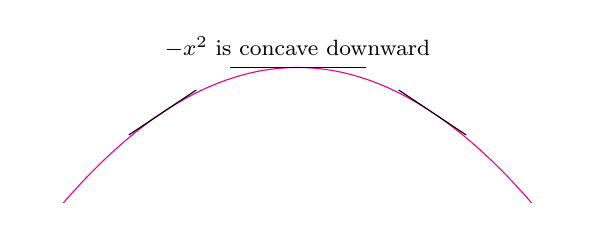
\begin{tikzpicture}
    \begin{axis}[
      axis lines=none,
      samples=500,
      smooth,
      no markers,
      xmin=-2, xmax=2,
      ymin=-1, ymax=1,
      ]
      % sage: f(x) = ((x+1)*(x-2)).integrate(x).integrate(x)
      \addplot[magenta] {-x^2/3};
      \addplot[domain=-0.5:0.5] {0};
      \addplot[domain=0.75:1.25] {-(2*x - 1)/3};
      \addplot[domain=-0.75:-1.25] {-(-2*x - 1)/3};
      \node[above] at (0,0) {\footnotesize \(-x^{2}\) is concave downward};
    \end{axis}
  \end{tikzpicture}
\end{document}
